
\section{The \BaFePAs series}

The \BaFePAs series is one of many that stem from the parent compount \BaFeAs, although unlike the electron doped \BaCoFeAs and the hole doped \BaKFeAs series, the \BaFePAs progression is entirely isovalent meaning that the changes affected due to the P substitution are due to structure and chemical pressure rather than additional charge carriers. Nonetheless, superconductivity occurs with a very similar phase diagram as with the charge-doped examples in the same `$122$' family of iron-pnictide materials.\footnote{See for example \Fig1 in ref.\cite{Paglione2010}}

At $x=0$ the \BaFePAs series begins at \BaFeAs, a compound which becomes antiferromagnetic at around \unit[138]{K}, and moves with increasing $x$ towards \BaFeP which is metallic to low temperatures. Neither end members are superconducting, however as As is substituted for P, the low temperature antiferromagnetic state decays, giving way to superconductivity which kicks in at approximately $x=0.18$ and increases to the optimal substitution of $x=0.31$. Superconductivity then decreases until it gives way to a paramagnetic ground state at around $x=0.71$. \Fig\ref{Fig:ResD:PhaseDiagram} shows the phase diagram adapated from ref. \cite{Nakai2010a} as determined by resistivity measurements. 
\begin{figure}[htbp]
    \begin{center}
        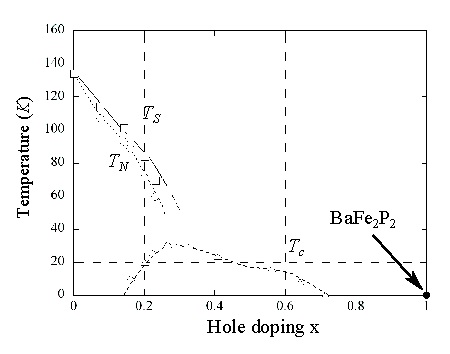
\includegraphics[scale=1.0]{Chapter-dHvABaFe2P2/Figures/BaFe2P2Series/PhaseDiagram/PhaseDiagram}
        \caption{Phase diagram adapted from ref \cite{Nakai2010a} measured by resistivity. $T_s$, $T_N$ and $T_c$ are the structural transition, the antiferromagnetic transition and the superconducting transition temperatures respectively.}
        \label{Fig:ResD:PhaseDiagram}
    \end{center}
\end{figure}
Also detailed in the phase diagram is the structural transition which occurs as the tetragonal $I4/mmm$ cell moves to an orthorhombic cell as it passes below the line marked $T_s$. This is a feature which is common to many of the `$122$' pnictide materials.

 The progression along the series is isovalent since P and As are in the same periodic group -- group $V$. The net effect of the substitution is to apply an increasing chemical pressure as $x$ moves towards $1$. Several reports show that applying \textit{physical} pressure to \BaFeAs results in a similar phase diagram with an antiferromagnetic phase and superconductivity up to $\sim$\unit[30]{K}\cite{Yamazaki2010,Colombier2009,Alireza2009} with Klintberg \textit{et al.}\cite{Klintberg2010} presenting a direct comparison between the two types of pressure. As pressure is applied, the unit cell $a$ axis shrinks slightly less than the $c$ axis ($\sim3\%$ c.f. $\sim4.5\%$ respectively). Interestingly the $c$ axis shrinking largely occurs in the Fe-Pnictide plane leading to some theories of the superconductivity emerging from the tetrahedral bond angle between the Fe and the pnictigen. \TODO{ref read Kuroki}
\begin{figure}[htbp]
    \begin{center}
        
\includegraphics[scale=1.0]{Chapter-dHvABaFe2P2/Figures/BaFe2P2Series/UnitCell/UnitCell}
        \caption{The tetragonal unit cell of the 122 \BaFePAs series.}
        \label{Fig:ResD:UnitCell}
    \end{center}
\end{figure}


The \BaFePAs series from a substitution of $x=0.41$--$1.0$ has been previously measured by members of the group at Bristol using dHvA oscillations\cite{Shishido2010}. As suggested in the Shishido reference, since dHvA has been observed across such a large range of substitutions, it implies that the material is not prone to disorder as is the case in many charge doped series \TODO{Need ref} making the series an excellant candidate for dHvA studies. The Fermi surfaces have been characterised for x ranging from $0.41$ to $1$ for electron sheets only but have clearly shown that the DFT calculations consistently overestimate the size of the surfaces. Moreover, dHvA measurements on the material with $x=0.63$ have been performed where one of the hole surface extrema was observed\cite{Analytis2010c} however DFT calculations as well as comparisons with \SrFeP\cite{Analytis2009} give evidence for a second hole Fermi surface for materials towards the P end of the series, (towards the As end of the series, there appears this second hole and a \textit{third} hole surface similar but smaller to the other hole sheets). If the electron Fermi surfaces are oversized in the DFT calculations, then the hole Fermi surface volumes should also be oversized in order to remain compensated (electrically neutral). What is not clear though is whether the \textit{shapes} of the hole pockets are also altered in the compounds leading to \BaFeP. DFT calculations show the larger of the hole pockets in particular undergoing significant geometric changes, specifically in that it becomes much more three dimensional as P substitution becomes more complete. The Fermi surface of the opposite end-member, \BaFeAs, has been fully characterised by previous ARPES measurements\cite{Kondo2010a} and dHvA\cite{Terashima2011, Analytis2010b}. Coupled with a full characterisation of the fermiology of \BaFeP, this data can be used to interpolate Fermiology of the hole pockets between end members thus completing the partial determination of the Fermi surfaces of the intermediary compounds.

The ARPES measurements of the Fermi surface of \BaFeAs below the N\'eel temperature concluded that despite some $k_z$ dispersion in the Fermi surfaces, there is adequate nesting to form the antiferromagnetic state. Ab-initio DFT calculations\cite{Shishido2010} of the paramagnetic state have shown the $k_z$ dispersion increasing with increasing P, with the outer hole pockets becoming more three-dimensional through the progression providing the partial nesting conditions necessary for pair forming SDW fluctuations described in section\ref{Sec:1:Nesting}. One caveat is that these calculations do not take into account the structural changes below $T_s$, another caveat is that they do not consider Fermi surface reconstruction due to the observed commensurate antiferromagnetic order. To fully settle the issue of the nature of the nesting in the superconducting state, experimental determination of the Fermi surfaces of the series is necessary, a good guide to which can be obtained from study of the end-members.


This thesis presents data which details the full Fermi surface of \BaFeP including an elucidation of the shape of the 3D outer hole surface. Partial nesting is detailed between the outer hole surface and the inner electron surface with $q=(\pi, \pi, \pi/2)$ meaning the phenomenum persists through to the end member of the series. Also presented are effective mass measurements which show relatively small mass enhancements implying weak carrier correlations.
